%%%%%%%%%%%%%%%%%%%%%%%%%%%%%%%%%%%%%%%%%%%%%%%%%%%%%%%%%%%%%%%%%
% MUW Presentation
% LaTeX Template
% Version 1.0 (27/12/2016)
%
% License:
% CC BY-NC-SA 4.0 (http://creativecommons.org/licenses/by-nc-sa/3.0/)
%
% Created by:
% Nicolas Ballarini, CeMSIIS, Medical University of Vienna
% nicoballarini@gmail.com
% http://statistics.msi.meduniwien.ac.at/
%
% Customized for UAH by:
% David F. Barrero, Departamento de Automática, UAH
%%%%%%%%%%%%%%%%%%%%%%%%%%%%%%%%%%%%%%%%%%%%%%%%%%%%%%%%%%%%%%%%%

\documentclass[10pt,compress]{beamer} % Change 10pt to make fonts of a different size
\mode<presentation>

\usepackage[spanish]{babel}
\usepackage{fontspec}
\usepackage{tikz}
\usepackage{etoolbox}
\usepackage{xcolor}
\usepackage{xstring}
\usepackage{listings}

% Custom packages
\usepackage{hhline} % Confusion matrix
\usepackage{multicol}
\usepackage{multirow} % Confusion matrix
\usepackage{tikz}
\usepackage{pgfplots}
\def\layersep{2.5cm}
\usetikzlibrary{matrix,chains,positioning,decorations.pathreplacing,arrows,shapes}

\definecolor{dkgreen}{rgb}{0,0.6,0}
\definecolor{gray}{rgb}{0.5,0.5,0.5}
\definecolor{mauve}{rgb}{0.58,0,0.82}
 

\usetheme{UAH}
\usecolortheme{UAH}
\setbeamertemplate{navigation symbols}{} 
\setbeamertemplate{caption}[numbered]

%%%%%%%%%%%%%%%%%%%%%%%%%%%%%%%%%%%%%%%%%%%%%%%%%%%%%%%%%%%%%%%%%
%% Presentation Info
\title[Machine Learning Foundations]{Machine Learning Foundations}
\author{\asignatura\\\carrera}
\institute{}
\date{Departamento de Automática}
%%%%%%%%%%%%%%%%%%%%%%%%%%%%%%%%%%%%%%%%%%%%%%%%%%%%%%%%%%%%%%%%%


%%%%%%%%%%%%%%%%%%%%%%%%%%%%%%%%%%%%%%%%%%%%%%%%%%%%%%%%%%%%%%%%%
%% Descomentar para habilitar barra de navegación superior
\setNavigation
%%%%%%%%%%%%%%%%%%%%%%%%%%%%%%%%%%%%%%%%%%%%%%%%%%%%%%%%%%%%%%%%%

%%%%%%%%%%%%%%%%%%%%%%%%%%%%%%%%%%%%%%%%%%%%%%%%%%%%%%%%%%%%%%%%%
%% Configuración de logotipos en portada
%% Opacidad de los logotipos
\newcommand{\opacidad}{1}
%% Descomentar para habilitar logotipo en pié de página de portada
\renewcommand{\logoUno}{Images/isg.png}
%% Descomentar para habilitar logotipo en pié de página de portada
%\renewcommand{\logoDos}{Images/CCLogo.png}
%% Descomentar para habilitar logotipo en pié de página de portada
%\renewcommand{\logoTres}{Images/ALogo.png}
%% Descomentar para habilitar logotipo en pié de página de portada
%\renewcommand{\logoCuatro}{Images/ELogo.png}
%%%%%%%%%%%%%%%%%%%%%%%%%%%%%%%%%%%%%%%%%%%%%%%%%%%%%%%%%%%%%%%%%

%%%%%%%%%%%%%%%%%%%%%%%%%%%%%%%%%%%%%%%%%%%%%%%%%%%%%%%%%%%%%%%%%
%% FOOTLINE
%% Comment/Uncomment the following blocks to modify the footline
%% content in the body slides. 


%% Option A: Title and institute
\footlineA
%% Option B: Author and institute
%\footlineB
%% Option C: Title, Author and institute
%\footlineC
%%%%%%%%%%%%%%%%%%%%%%%%%%%%%%%%%%%%%%%%%%%%%%%%%%%%%%%%%%%%%%%%%


% This is for the confusion matrix, DELETE if not needed
\def\colorModel{hsb} %You can use rgb or hsb

\newcommand\ColCell[1]{
   \pgfmathparse{#1<50?1:0}  %Threshold for changing the font color into the cells
       \ifnum\pgfmathresult=0\relax\color{white}\fi
   \pgfmathsetmacro\compA{0}      %Component R or H
   \pgfmathsetmacro\compB{#1/100} %Component G or S
   \pgfmathsetmacro\compC{1}      %Component B or B
   \edef\x{\noexpand\centering\noexpand\cellcolor[\colorModel]{\compA,\compB,\compC}}\x #1
} 
%\newcolumntype{E}{>{\collectcell\ColCell}m{0.4cm}<{\endcollectcell}}  %Cell width
\newcommand*\rot{\rotatebox{90}}


\begin{document}

%%%%%%%%%%%%%%%%%%%%%%%%%%%%%%%%%%%%%%%%%%%%%%%%%%%%%%%%%%%%%%%%%
% Use this block for a blue title slide with modified footline
{\titlepageBlue
    \begin{frame}
        \titlepage
    \end{frame}
}

\institute{\asignatura}

\begin{frame}[plain]{}
   \begin{block}{Objectives}
      \begin{enumerate}
         \item Define Machine Learning (ML)
		 \item Delimite ML scope
         \item Introduce the main ML tasks
         \item Recognize problems as ML tasks
      \end{enumerate} 
   \end{block}

   \begin{block}{Bibliography}
	\begin{itemize}
        \item Bishop, Christopher M. \textit{Pattern Recognition and Machine Learning}. 2nd edition. Springer-Verlag. 2011
        \item M\"uller, Andreas C., Guido, Sarah. \textit{Introduction to Machine Learning with Python}. O'Reilly. 2016
	\end{itemize}
   \end{block}
\end{frame}

{
\disableNavigation{white}
\begin{frame}[shrink]{Table of Contents}

 	\frametitle{Table of Contents}
  	\begin{multicols}{2}
  		\tableofcontents
    \end{multicols}

 %\frametitle{Table of Contents}
 %\tableofcontents
  % You might wish to add the option [pausesections]
\end{frame}
}

\section{Introduction}

\subsection{Justification}
\begin{frame}{Introduction}{Justification}
	 New opportunities
	\begin{itemize}
	\item Huge amount of new data sources: banking, social media, IoT, DNA, ...
	\item Increased computational power
	\end{itemize}
	New needs
	\begin{itemize}
	\item Manual data analysis is unfeasible
	\item Need of automatic methods
	\end{itemize}
	New goal
	\begin{itemize}
		\item Transform data into knowledge
	\end{itemize}
\end{frame}

\subsection{Definition}
\begin{frame}{Introduction}{Definition (I)}

	\begin{columns}
 	   \column{.60\textwidth}
	   \begin{block}{ML definition}
		ML is the science (and art) of programming computers so they can \textit{learn from data}.

		\hfill A. G\'eron, 2017
		\end{block}
	\end{columns}

	\bigskip

	Alternative definitions
	\begin{itemize}
	\item Machine Learning is the field of study that gives computers the ability to learn without being explicitly programmed. Arthur Samuel, 1959.
	\item A computer program is said to learn from experience E with respect to some task T and some performance measure P, if its performance on T, as measured by P, improves with experience. E. Tom Mitchell, 1997.
	\end{itemize}
\end{frame}

\begin{frame}{Introduction}{Definition (II)}
	\begin{center}
	\textbf{Traditional approach}\\
	
\usetikzlibrary{arrows,positioning,backgrounds}

\tikzstyle{decision} = [diamond, draw, 
    text width=1cm, text badly centered, node distance=3cm, inner sep=0pt]
\tikzstyle{block} = [rectangle, draw, node distance=3cm,
	    text width=2cm, text centered, rounded corners]
\tikzstyle{line} = [draw, -latex']

\begin{tikzpicture}[scale=0.8]
	\node [block] (problem) {Study problem};
	\node [block, right of=problem] (center) {Write rules};
	\node [decision, right of=center] (evaluate) {Evaluate};
	\node [block, below of=center, node distance=1cm] (errors) {Analyze errors};
	\node [block, above of=evaluate, node distance=1cm] (launch) {Launch!};

	\path [line] (problem) -- (center);
	\path [line] (center) -- (evaluate);
	\path [line] (evaluate) -- (launch);
	\path [line] (evaluate) |- (errors);
	\path [line] (errors) -| (problem);
\end{tikzpicture}
\\
	\bigskip
	\textbf{ML approach}\\
	
\usetikzlibrary{arrows,positioning,backgrounds}

\tikzstyle{decision} = [diamond, draw, 
    text width=1cm, text badly centered, node distance=3cm, inner sep=0pt]
\tikzstyle{block} = [rectangle, draw, node distance=3cm,
	    text width=2cm, text centered, rounded corners]
\tikzstyle{line} = [draw, -latex']

\begin{tikzpicture}[scale=0.8]
	\node [block] (problem) {Study problem};
	\node [block, right of=problem] (center) {Train};
	\node [decision, right of=center] (evaluate) {Evaluate};
	\node [block, below of=center, node distance=1cm] (errors) {Analyze errors};
	\node [block, above of=evaluate, node distance=1cm] (launch) {Launch!};
	\node [block, trapezium, trapezium left angle=70,trapezium right angle=-70, above of=center, node distance=1cm, text width=0.7cm] (data) {Data};

	\path [line] (problem) -- (center);
	\path [line] (center) -- (evaluate);
	\path [line, dotted] (data) -- (center);
	\path [line] (evaluate) -- (launch);
	\path [line] (evaluate) |- (errors);
	\path [line] (errors) -| (problem);
\end{tikzpicture}

	\end{center}	
\end{frame}

\subsection{The alphabet soup of data analysis}
\begin{frame}{Introduction}{The alphabet soup of data analysis}
	\begin{center}
	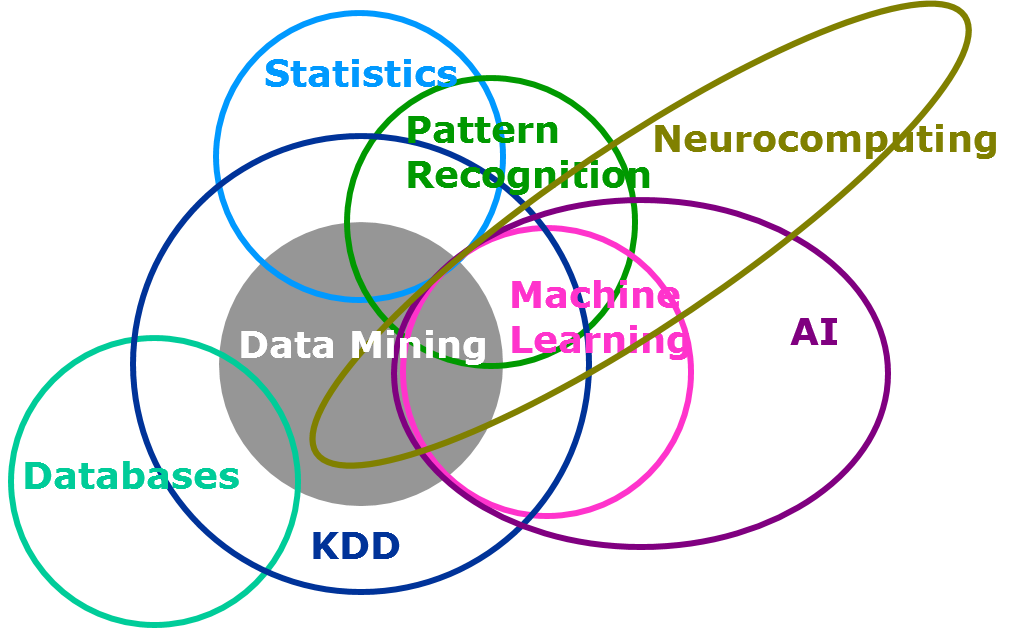
\includegraphics[width=0.5\linewidth]{figs/terms.png}\\
    \tiny{\href{https://www.quora.com/What-is-machine-learning-and-how-it-is-linked-to-Big-Data-Data-Mining}{(Source)}}
	\end{center}

	Many related terms:

    \begin{columns}
 	   \column{.30\textwidth}
		\begin{itemize}
		\item Big Data
		\item Data Science
		\item Business Intelligence
		\end{itemize}
 	   \column{.30\textwidth}
		\begin{itemize}
		\item Data Mining
		\item Deep Learning
		\item Predictive analytics
		\item KDD
		\end{itemize}
 	   \column{.30\textwidth}
		\begin{itemize}
		\item Data scientist
		\item Data engineer
		\item ML engineer
		\end{itemize}
    \end{columns}
\end{frame}

\section{The data analysis process}
\subsection{The big picture}
\begin{frame}{The data analysis process}{The big picture}
	\begin{center}
	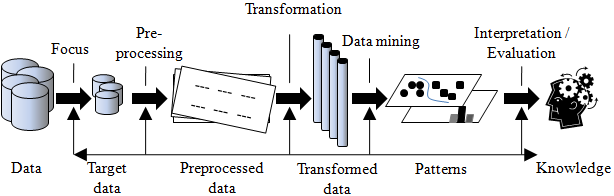
\includegraphics[width=0.8\linewidth]{figs/kdd.png}\\
    \tiny{\href{https://www.researchgate.net/figure/The-steps-of-the-KDD-process_fig6_297734487}{(Source)}}
	\end{center}

	\begin{columns}
 	   \column{.60\textwidth}
		Steps in any ML application:
		\begin{enumerate}
			\item Data adquisition
			\item Selection, cleaning and transformation
			\item Machine Learning
			\item Learning evaluation
			\item Explotation
		\end{enumerate}

 	  \column{.40\textwidth}
	   \begin{block}{}
	   		The goal in ML is to get a representation of those patterns
	   \end{block}
	\end{columns}
\end{frame}

\subsection{Data adquisition}
\begin{frame}{The data analysis process}{Data adquisition}
	Goal: Adquire data to perform ML
		\begin{itemize}
		\item From extremely easy -CSV file- to extremely complex -full Big Data system-
		\end{itemize}

	Public data repositories
		\begin{itemize}
		\item \href{https://www.kaggle.com/}{(Kaggle)}, \href{https://data.nasa.gov/}{(NASA Open Data Portal)} \IfStrEq{\modo}{mcyte}{, \href{https://omniweb.gsfc.nasa.gov/}}{(Omniweb)}{},\href{https://archive.ics.uci.edu/ml/index.php}{(UCI Machine Learning Repository)}
		\end{itemize}
	Customized adquisition and integration
		\begin{itemize}
		\item Integration from several data sources usually needed
		\end{itemize}

		\begin{figure}
		\centering{
		\resizebox{0.6\textwidth}{!}{\input{figs/integration.pdf_tex}}}
		\end{figure}
\end{frame}

\subsection{Selection, cleaning and transformation}
\begin{frame}{The data analysis process}{Selection, cleaning and transformation (I)}
	\begin{columns}
 	   \column{.60\textwidth}
	Goal: Prepare data for ML
		\begin{itemize}
		\item This phase is usually named \alert{preprocess}
		\end{itemize}

	ML requires a clean data table
	 \begin{itemize}
	 	\item Rows are named \alert{instances}
		\item Columns are named \alert{features} or \alert{attributes}
		\item We refer the number of features as \alert{dimensionality}
	 \end{itemize}
	In some ML problems we use graphs instead of tables

 	   \column{.40\textwidth}
		\begin{center}
		\begin{tabular}{cccc}\hline
		 	$f_1$     & $f_2$     & $\cdots$ & $f_n$     \\\hline
		 	$a_{1,1}$ & $a_{2,1}$ & $\cdots$ & $a_{n,1}$ \\
		 	$a_{1,2}$ & $a_{2,2}$ & $\cdots$ & $a_{n,2}$ \\
		 	$a_{1,3}$ & $a_{2,3}$ & $\cdots$ & $a_{n,3}$ \\
		 	$a_{1,4}$ & $a_{2,4}$ & $\cdots$ & $a_{n,4}$ \\
		 	$a_{1,5}$ & $a_{2,5}$ & $\cdots$ & $a_{n,5}$ \\
		 	\hline
		\end{tabular}
		\end{center}
	\end{columns}
\end{frame}

\begin{frame}[fragile]{The data analysis process}{Selection, cleaning and transformation (II)}
	\begin{exampleblock}{Example: Bank data base}
	 \vspace{-0.3cm}
	\begin{center}
	\begin{tabular}{cccccc}\hline
		 \texttt{IDC} & \texttt{Years}& \texttt{Euros} & \texttt{Salary} & \texttt{Own house} & \texttt{Defaults} \\\hline
		 101 & 15   & 60000 & 2200   & Yes       & 2   \\
		 102 & 2    & 30000 & 3500   & Yes       & 0   \\
		 103 & 9    & 9000  & 1700   & Yes       & 1   \\
		 104 & 15   & 18000 & 1900   & No        & 0   \\
		 $\cdots$ & $\cdots$ & $\cdots$ & $\cdots$   & $\cdots$ & $\cdots$ \\
		 \hline
	 \end{tabular}
	 \end{center}
	 \vspace{-0.4cm}
	 \end{exampleblock}

	\begin{exampleblock}{Example: Robot sensors}
	 \vspace{-0.3cm}
	\begin{center}
	\begin{tabular}{cccccc}\hline
		 \texttt{Timestamp}	& \texttt{Sonar1} & \texttt{Sonar2} & \texttt{Sonar3} & \texttt{Sonar4}  \\\hline
		 1 			& 1.687	 & 0.445  & 2.332  & 0.429   \\
		 2 			& 0.812	 & 0.481  & 1.702  & 0.473   \\
		 3 			& 1.572  & 0.471  & 1.654  & 0.513   \\
		 $\cdots$   & $\cdots$& $\cdots$& $\cdots$ & $\cdots$ \\
		 \hline
	 \end{tabular}
	 \end{center}
	 \vspace{-0.4cm}
	 \end{exampleblock}
\end{frame}

\begin{frame}[fragile]{The data analysis process}{Selection, cleaning and transformation (III)}
	\begin{exampleblock}{Example: Image recognition}
	 \vspace{-0.3cm}
	%\begin{columns}
 	 %  \column{.50\textwidth}
		\begin{center}
		
\includegraphics[width=0.5\linewidth]{figs/8-Digit-Recognition}\\
    	\tiny{\href{https://lucenaresearch.com/deep-neural-networks/}{(Source)}}
		\end{center}

 	  % \column{.50\textwidth}
		\begin{center}
		\begin{tabular}{ccccc}\hline
		 \texttt{Pixel1}& \texttt{Pixel2} & \texttt{Pixel3} & $\cdots$ & \texttt{Pixel784} \\\hline
		 0     & 0      & 0      & $\cdots$ & 0                  \\
		 $\cdots$ & $\cdots$ & $\cdots$ & $\cdots$   & $\cdots$  \\
		 0     & 0      & 0      & $\cdots$ & 0                  \\
		 \hline
	 	\end{tabular}
	 	\end{center}
	 %\end{columns}
	 \vspace{-0.3cm}
	 \end{exampleblock}
\end{frame}

\begin{frame}[fragile]{The data analysis process}{Selection, cleaning and transformation (IV)}
	\begin{exampleblock}{Example: Text classification (bag-of-words representation)}
	 \vspace{-0.2cm}
	\begin{enumerate}
		\item Original text\\
		\begin{lstlisting}[basicstyle=\scriptsize]
(1) John likes to watch movies. Mary likes movies too.
(2) John also likes to watch football games.
\end{lstlisting}
		\item Build list\\
		\begin{lstlisting}[language=Python,basicstyle=\tiny]
(1) "John","likes","to","watch","movies","Mary","likes","movies","too"
(2) "John", also","likes","to","watch","football","games"
\end{lstlisting}
		\item Build dictionary\\
		\begin{lstlisting}[language=Python,basicstyle=\tiny]
(1) {"John":1,"likes":2,"to":1,"watch":1,"movies":2,"Mary":1,"too":1};
(2) {"John":1,"also":1,"likes":1,"to":1,"watch":1,"football":1,"games":1};
\end{lstlisting}
	\end{enumerate}

	 \vspace{-0.5cm}

	\begin{center}
	\begin{tabular}{cccccccccc}\hline
		 John & likes & to & watch & movies & Mary & too & also & games & $\cdots$ \\\hline
		 1    & 2     & 1  & 1     & 2      & 1    & 1   & 0 	& 0 	& $\cdots$ \\
		 1    & 1     & 1  & 1     & 0      & 0    & 0   & 1 	& 1 	& $\cdots$ \\
		 \hline
	 \end{tabular}
	 \end{center}
	 \vspace{-0.4cm}
	 \end{exampleblock}
\end{frame}

\begin{frame}{The data analysis process}{Selection, cleaning and transformation (V)}
	Preprocessing tasks
		\begin{itemize}
		\item Handle outliers (remove or leave them)
		\item Sample data (in case there are too much)
		\item Handle missing values
		\item Remove irrelevant or redundant features (\alert{feature selection})
			\begin{itemize} 
			\item For instance, attributes ``social class'' and ``salary'' contain highly correlated information
			\end{itemize}
		\item Compute new attributes (\alert{feature engineering})
			\begin{itemize}
			\item For instance, compute ``population density'' from ``area'' and ``population''
			\end{itemize}
		\item Transform attributes
			\begin{itemize}
				\item Discretization, normalization, numerization, ...
			\end{itemize}
		\end{itemize}
\end{frame}

\IfStrEq{\modo}{mcyte}{
\begin{frame}{The data analysis process}{Data processing levels}
	Three levels of processing for data products
	\begin{itemize}
		\item Level 0: Unprocessed data from payload
		\item Level 1: Processed data
		\item Level 2: Processed data with geophysical variables
	\end{itemize}

	\href{(https://science.nasa.gov/earth-science/earth-science-data/data-processing-levels-for-eosdis-data-products/}{(More info)}
\end{frame}
}{}

\subsection{Machine Learning}
\begin{frame}{The data analysis process}{Machine Learning}
	Goal: Train an algorithm to perform a task
		\begin{itemize}
		\item As result, we obtain a \alert{model} (or \alert{classifier} or \alert{predictor} depending on the context)
		\end{itemize}

	Machine Learning training methods (or ML tasks)
		\begin{itemize}
		\item Supervised learning: \textbf{classification} and regression
		\item Unsupervised learning: \textbf{clustering}, association, \textbf{dimensionality reduction} and anomality detection
        \item Reinforcement learning
		\item Many others
		\end{itemize}

	\vspace{-0.5cm}
	 \begin{flushright}
		\begin{columns}
 	   	\column{.25\textwidth}
 	   	\column{.50\textwidth}
		\begin{block}{No Free-Lunch Theorem}
		No learning algorithm is a priori guaranteed to work better\\
		More info: \href{http://citeseerx.ist.psu.edu/viewdoc/download?doi=10.1.1.390.9412&rep=rep1&type=pdf}{(D. Wolpert, 1996)}
		\end{block}
 	   	\column{.25\textwidth}
		\end{columns}
	 \end{flushright}

\end{frame}

\subsection{Learning evaluation}
\begin{frame}{The data analysis process}{Learning evaluation (I)}
	We do need to evaluate the trained model
	\begin{itemize}
		\item Models should perform well on new data
	\end{itemize}
	A na\"ive and wrong approach. Why is it wrong?
	\begin{enumerate}
		\item Train the model
		\item Use the model to predict labels
		\item Compute accuracy comparing predicted labels with known labels
	\end{enumerate}
	Solution: Training and validation datasets
	\begin{itemize}
		\item \textbf{Training set}: Data used to train the models. Usually 70\%
		\item \textbf{Validation set}: Data used to validate the models. Usually 30\%
		\item Problems: Bias and loose of relevant data (serious in small datasets)
	\end{itemize}
\end{frame}

\begin{frame}{The data analysis process}{Learning evaluation (II)}
	\begin{columns}
 	   \column{.50\textwidth}
		\begin{block}{Crossvalidation}
			\begin{enumerate}
			\item Divide dataset in folds
			\item Take one fold for validation
			\item Train with the other folds
			\item Validate and compute performance
			\item Take another fold and repeat until finish
			\item Average performance measures
		    \end{enumerate}
		\end{block}

		Usually we use 10 folds 
		\begin{itemize}
			\item 10-fold cross validation (or 10-CV)
		\end{itemize}

 	   \column{.50\textwidth}
		\begin{center}
		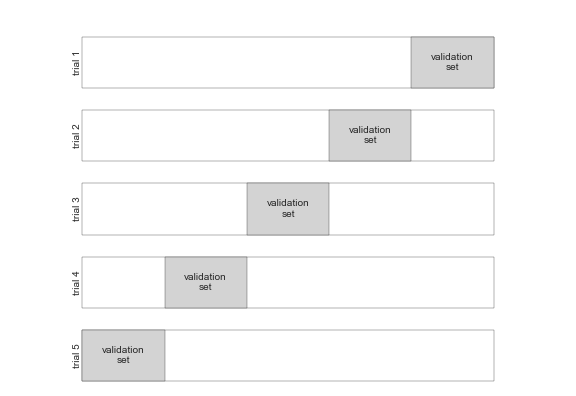
\includegraphics[width=\linewidth]{figs/05.03-5-fold-CV.png}\\
    	\tiny{\href{https://jakevdp.github.io/PythonDataScienceHandbook/05.03-hyperparameters-and-model-validation.html}{(Source)}}
		\end{center}
	\end{columns}
\end{frame}

\begin{frame}{The data analysis process}{Learning evaluation (III)}
	\begin{columns}
 	   \column{.50\textwidth}
            Select a measure to evaluate learning
            \begin{itemize}
                \item Proper measures depends on the problem
            \end{itemize}
            Classification learning measures
            \begin{itemize}
                \item Accuracy: Ratio of correct predictions
                \item F-Measure
                \item Confusion matrix
                \item ROC curve
            \end{itemize}
            Regression learning measures
            \begin{itemize}
                \item Mean Absolute Error (MAE)
                \item Mean Squared Error (MSE)
                \item $R^2$
            \end{itemize}

 	   \column{.50\textwidth}
    		\begin{alertblock}{}
                Validation error must be taken, always, on the validation set
	    	\end{alertblock}

        	\begin{block}{Confusion matrix}
                \newcommand\items{3}   %Number of classes
                %\arrayrulecolor{white} %Table line colors
                \noindent\begin{tabular}{cc*{\items}{|c}|}
                    \multicolumn{1}{c}{} &\multicolumn{1}{c}{} &\multicolumn{\items}{c}{\textit{Predicted class}} \\ %\hhline{~*\items{|-}|}
                    \multicolumn{1}{c}{} & 
                    \multicolumn{1}{c}{} & 
                    \multicolumn{1}{c}{\rot{Class A}} & 
                    \multicolumn{1}{c}{\rot{Class B}} & 
                    \multicolumn{1}{c}{\rot{Class C}} \\ \hhline{~~*\items{|-}|}
                    \multirow{\items}{*}{\rotatebox{90}{\textit{Actual class}}} 
                    &Class A  & 100   & 0  & 10   \\ \hhline{~~*\items{|-}|}
                    &Class B  & 10   & 80  & 10   \\ \hhline{~~*\items{|-}|}
                    &Class C  & 30   & 0   & 70   \\ \hhline{~~*\items{|-}|}
                \end{tabular}\\
                \tiny \href{https://tex.stackexchange.com/questions/20267/how-to-construct-a-confusion-matrix-in-latex}{(Source)}
	    	\end{block}
	\end{columns}
\end{frame}



\subsection{Model exploitation}
\begin{frame}{The data analysis process}{Model exploitation}
	Model explotation depends on the objectives
		\begin{itemize}
		\item In Data Science, the model is interpreted and a report wroten
			\begin{itemize}
				\item Formal report, bussiness intelligence dashboard, ...
			\end{itemize}
		\item In Machine Learning, the model is integrated into a software system
			\begin{itemize}
				\item Web application, app, robot controller, ...
			\end{itemize}
		\end{itemize}
	The model may need maintenance
\end{frame}

\section{Types of Machine Learning systems}
\subsection{Overview}

\begin{frame}{Types of Machine Learning systems}{Overview}
	We can classify ML systems based on several (non-exclusive) criteria
	\begin{itemize}
		\item Whether or not they are trained with human supervision
			\begin{itemize}
			\item Supervised, unsupervised, semisupervised and Reinforcement Learning
			\end{itemize}
		\item Whether or not they can learn incrementally
			\begin{itemize}
			\item Online vs. batch learning
			\end{itemize}
		\item Whether they compare new data to known data
			\begin{itemize}
			\item Instance-based vs. model-based learning
			\end{itemize}
		\item The purpose of the system
			\begin{itemize}
			\item Predictice models vs. explicative models
			\end{itemize}
		\item The goal of the system
			\begin{itemize}
			\item Discriminative models vs. generative models
			\end{itemize}
	\end{itemize}
	We focus on supervised and unsupervised model-based discriminative batch algorithms.
\end{frame}

\begin{frame}[fragile]{Types of Machine Learning systems}{Supervised learning (I)}
	In supervised learning input data comes along with the desired output
	\begin{itemize}
		\item Usually human beings label the output (named \alert{labels})
	\end{itemize}

	\begin{center}
	\begin{tabular}{cccccc}\hline
	 	$f_1$     & $f_2$     & $\cdots$ & $f_n$     & $y$\\\hline
	 	$a_{1,1}$ & $a_{2,1}$ & $\cdots$ & $a_{n,1}$ & $y_1$ \\
	 	$a_{1,2}$ & $a_{2,2}$ & $\cdots$ & $a_{n,2}$ & $y_2$ \\
	 	$a_{1,3}$ & $a_{2,3}$ & $\cdots$ & $a_{n,3}$ & $y_3$ \\
	 	$a_{1,4}$ & $a_{2,4}$ & $\cdots$ & $a_{n,4}$ & $y_4$ \\
	 	$a_{1,5}$ & $a_{2,5}$ & $\cdots$ & $a_{n,5}$ & $y_5$ \\
	 	\hline
	\end{tabular}
	\end{center}

	 Two main tasks in supervised learning
	 \begin{itemize}
	 	\item \textbf{Classification} if $y$ is a categorical attribute. Target attribute named \alert{class}
		\item \textbf{Regression} if $y$ is numerical 
	 \end{itemize}
	 Advanced supervised learning tasks
	\begin{itemize}
	 	\item Semi-supervised learning, weakly supervised learning and multilabel classification
	 \end{itemize}

\end{frame}

\begin{frame}{Types of Machine Learning systems}{Supervised learning (II)}
	\vspace{-0.25cm}
	\begin{columns}
 	   \column{.50\textwidth}
	   \centering Classification\\
			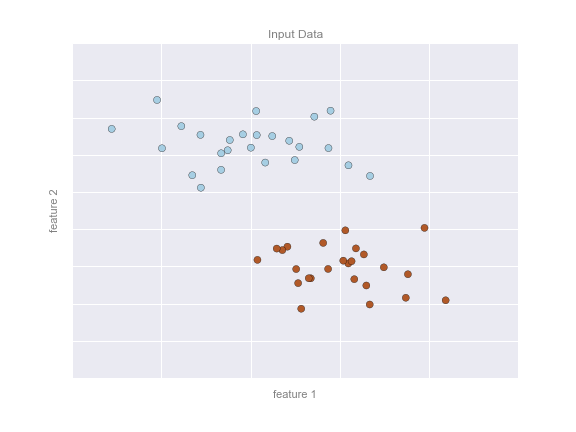
\includegraphics[width=0.8\linewidth]{figs/05.01-classification-1.png}\\
			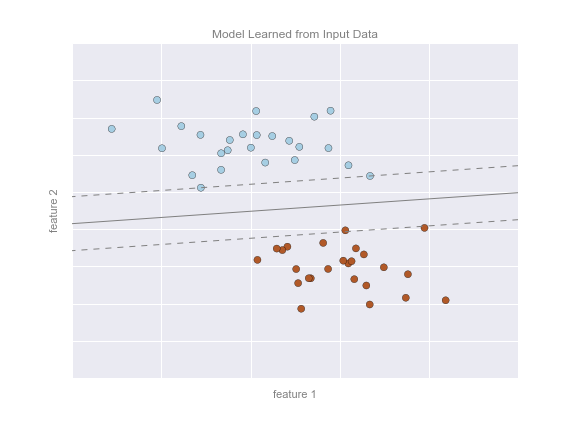
\includegraphics[width=0.8\linewidth]{figs/05.01-classification-2.png}\\
    		\tiny{\href{https://jakevdp.github.io/PythonDataScienceHandbook/05.01-what-is-machine-learning.html}{(Source)}}
 	   \column{.50\textwidth}
	   \centering Regression
			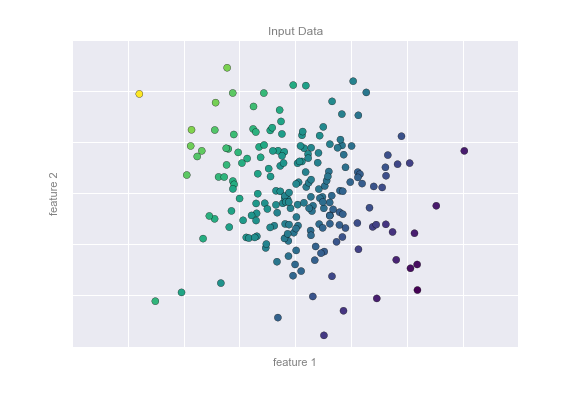
\includegraphics[width=0.8\linewidth]{figs/05.01-regression-1.png}\\
			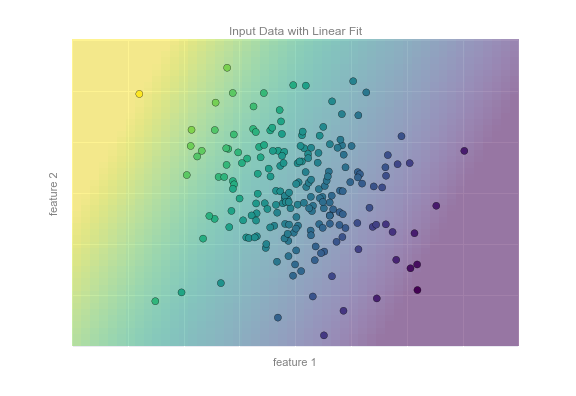
\includegraphics[width=0.8\linewidth]{figs/05.01-regression-3.png}\\
    		\tiny{\href{https://jakevdp.github.io/PythonDataScienceHandbook/05.01-what-is-machine-learning.html}{(Source)}}
	\end{columns}
\end{frame}

\begin{frame}{Types of Machine Learning systems}{Supervised learning (III)}
	\begin{columns}
 	   \column{.50\textwidth}
	   Important \textit{classification} algorithms:
	   \begin{itemize}
	   		\item k-Nearest Neighbors
			\item Support Vector Machines (SVMs)
			\item Decision Trees
				\begin{itemize}
				\item ID3, C4.5 (J48), ...
				\end{itemize}
			\item Rules
				\begin{itemize}
				\item PART, CN2, AQ, ...
				\end{itemize}
			\item Random Forests
			\item Bayesian Networks
			\item Neural Networks
			\item Ensambles
	   \end{itemize}
 	   \column{.50\textwidth}
	   Important \textit{regression} algorithms:
	   \begin{itemize}
	   		\item Linear Regression
			\item Logistic Regression
			\item Symbolic Regression
			\item Regression trees
				\begin{itemize}
				\item LM3 (M5), ...
				\end{itemize}
			\item Neural Networks
	   \end{itemize}
	\end{columns} 
\end{frame}

\subsection{Classification}
\begin{frame}{Types of Machine Learning systems}{Supervised learning: Classification (I)}
	Example: Bank credit risk management

	\begin{center}
	\begin{tabular}{ccccccc}\hline
		 IDC & Years& Euros & Salary & Own house & Defaulter accounts & \textit{Returns credit} \\\hline
		 101 & 15   & 60000 & 2200   & Yes       & 2                  & \textit{No} \\
		 102 & 2    & 30000 & 3500   & Yes       & 0                  & \textit{Yes} \\
		 103 & 9    & 9000  & 1700   & Yes       & 1                  & \textit{No} \\
		 104 & 15   & 18000 & 1900   & No        & 0                  & \textit{Yes} \\
		 105 & 10   & 24000 & 2100   & No        & 0                  & \textit{No} \\
		 $\cdots$ & $\cdots$ & $\cdots$ & $\cdots$   & $\cdots$  & $\cdots$ & $\cdots$ \\
		 \hline
	 \end{tabular}
	 \end{center}

	Objective: Predict if a customer would return a credit or not
\end{frame}

\begin{frame}{Types of Machine Learning Systems}{Supervised learning: Classification (II)}
	\begin{figure}[h]
	\centering{
		\resizebox{\textwidth}{!}{\input{figs/bankclassification.pdf_tex}}}
	\end{figure}
\end{frame}

\begin{frame}{Types of Machine Learning systems}{Supervised learning: Classification (III)}
	Example: Cancerous cells prediction
	\begin{columns}
 	   \column{.10\textwidth}
 	   \column{.20\textwidth}
			\begin{figure}
			\centering{
			\resizebox{0.9\textwidth}{!}{\input{figs/cells.pdf_tex}}}
			\end{figure}

 	   \column{.70\textwidth}

		\begin{center}
		\begin{tabular}{ccccc}\hline
		 \texttt{ID} & \texttt{Colour} & \texttt{nuclei}& \texttt{tails} & \texttt{\textit{class}} \\\hline
		 H1 & light  & 1     & 1     & \textit{healthy} \\
		 H2 & dark   & 1     & 1     & \textit{healthy} \\
		 H3 & light  & 1     & 2     & \textit{healthy} \\
		 H4 & light  & 2     & 1     & \textit{healthy} \\
		 C1 & dark   & 1     & 2     & \textit{cancer} \\
		 C2 & dark   & 2     & 1     & \textit{cancer} \\
		 C3 & light  & 2     & 2     & \textit{cancer} \\
		 C4 & dark   & 2     & 2     & \textit{cancer} \\
		 \hline
	 	\end{tabular}
	\end{center}
	\end{columns}
\end{frame}

\begin{frame}[fragile]{Types of Machine Learning systems}{Supervised learning: Classification (IV)}
	Example: Cancerous cells prediction
	\begin{columns}
 	   \column{.10\textwidth}
 	   \column{.20\textwidth}
			\begin{figure}
			\centering{
			\resizebox{0.9\textwidth}{!}{\input{figs/cells.pdf_tex}}}
			\end{figure}

 	   \column{.70\textwidth}
	   		\begin{exampleblock}{Decision rules}
	   		\begin{lstlisting}[firstnumber=1, xleftmargin=10pt] 
if colour = light  and  nuclei = 1 
then cell = healthy   	
			            
if nuclei = 2  and  colour = dark
then cell = cancerours

(and 4 rules more)
          \end{lstlisting}
	   		\end{exampleblock}
	\end{columns}
\end{frame}

\begin{frame}[fragile]{Types of Machine Learning systems}{Supervised learning: Classification (V)}
	Example: Cancerous cells prediction
	\begin{columns}
 	   \column{.10\textwidth}
 	   \column{.20\textwidth}
			\begin{figure}
			\centering{
			\resizebox{0.9\textwidth}{!}{\input{figs/cells.pdf_tex}}}
			\end{figure}

 	   \column{.70\textwidth}
	   		\begin{exampleblock}{Hierarchical decision rules}
	   		\begin{lstlisting}[firstnumber=1, xleftmargin=10pt]
if colour = light and nuclei = 1 
then cell = healthy   	
			            
else 
    if nuclei = 2 and colour = dark
    then cell = cancerous

   else 
        if tails = 1 
        then cell = healthy

        else cell = cancerous
       \end{lstlisting}
	   	\end{exampleblock}
	\end{columns}
\end{frame}

\begin{frame}[fragile]{Types of Machine Learning systems}{Supervised learning: Classification (VI)}
	Example: Cancerous cells prediction
	\begin{columns}
 	   \column{.10\textwidth}
 	   \column{.20\textwidth}
			\begin{figure}
			\centering{
			\resizebox{0.9\textwidth}{!}{\input{figs/cells.pdf_tex}}}
			\end{figure}

 	   \column{.50\textwidth}
	   		\begin{exampleblock}{Decision tree}
				\begin{figure}
				\centering{
				\resizebox{0.9\textwidth}{!}{\input{figs/tree.pdf_tex}}}
				\end{figure}
	   		\end{exampleblock}
 	   \column{.20\textwidth}
	\end{columns}
\end{frame}

\begin{frame}[fragile]{Types of Machine Learning systems}{Supervised learning: Classification (VII)}
	Example: Cancerous cells prediction
	\begin{columns}
 	   \column{.10\textwidth}
 	   \column{.20\textwidth}
			\begin{figure}
			\centering{
			\resizebox{0.9\textwidth}{!}{\input{figs/cells.pdf_tex}}}
			\end{figure}

 	   \column{.50\textwidth}
	   		\begin{exampleblock}{Neural network}
				\begin{figure}
				\centering{
				\resizebox{0.9\textwidth}{!}{\input{figs/nn.pdf_tex}}}
				\end{figure}
	   		\end{exampleblock}
 	   \column{.20\textwidth}
	\end{columns}
\end{frame}

\subsection{Regression}
\begin{frame}{Types of Machine Learning systems}{Supervised learning: Regression (I)}
	Example: Does money make people happier? (example from (G\'eron, 2017))
	\bigskip

	\begin{columns}
 	   \column{.40\textwidth}
		\begin{tabular}{ccc}\hline
		 	\texttt{Country} & \texttt{GDP} & \texttt{\textit{LS}} \\\hline
		 	Hungary& 12,240  & \textit{4.9}   \\
		 	Korea 	& 27,195  & \textit{5.8}   \\
		 	France & 37,675  & \textit{6.5}   \\
		 	Australia & 50,962 & \textit{7.3} \\
		 	USA 	& 55,805  & \textit{7.2}   \\
		 	\hline
	 	\end{tabular}\\
		LS =Life satisfaction

 	   \column{.60\textwidth}
	   		\begin{exampleblock}{Linear regression}
				\centering 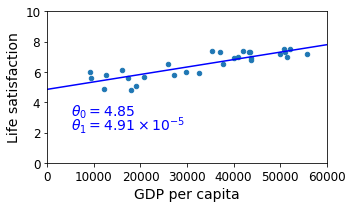
\includegraphics[width=0.9\linewidth]{figs/scattergdpregression.png}
				\vspace{-0.4cm}
				\begin{equation*}
				life\_satisfaction = \theta_0 + \theta_1 \times GDP\_per\_capita
				\end{equation*}
				\vspace{-0.2cm}
	   		\end{exampleblock}
	\end{columns}
\end{frame}

\subsection{Unsupervised learning}
\begin{frame}{Types of Machine Learning systems}{Unsupervised learning}
	In unsupervised learning there are no labels

	\begin{center}
	\begin{tabular}{ccccc}\hline
		 $f_1$     & $f_2$     & $f_3$     & $\cdots$ & $f_n$     \\\hline
		 $a_{1,1}$ & $a_{2,1}$ & $a_{3,1}$ & $\cdots$ & $a_{n,1}$ \\
		 $a_{1,2}$ & $a_{2,2}$ & $a_{3,2}$ & $\cdots$ & $a_{n,2}$ \\
		 $a_{1,3}$ & $a_{2,3}$ & $a_{3,3}$ & $\cdots$ & $a_{n,3}$ \\
		 $a_{1,4}$ & $a_{2,4}$ & $a_{3,4}$ & $\cdots$ & $a_{n,4}$ \\
		 $a_{1,5}$ & $a_{2,5}$ & $a_{3,5}$ & $\cdots$ & $a_{n,5}$ \\
		 \hline
	 \end{tabular}
	 \end{center}

	Tasks in unsupervised learning
	\begin{itemize}
		\item Clustering
		\item Association rules
		\item Dimensionality reduction
		\item Anomality detection
	\end{itemize}

\end{frame}

\subsection{Clustering}
\begin{frame}{Types of Machine Learning systems}{Unsupervised learning: Clustering (I)}
	Clustering is a set of techniques that identify groups of data
		\begin{itemize}
			\item Algorithms: K-means, Expectation Maximization (EM), ...
		\end{itemize}

    \begin{columns}
 	   \column{.50\textwidth}
			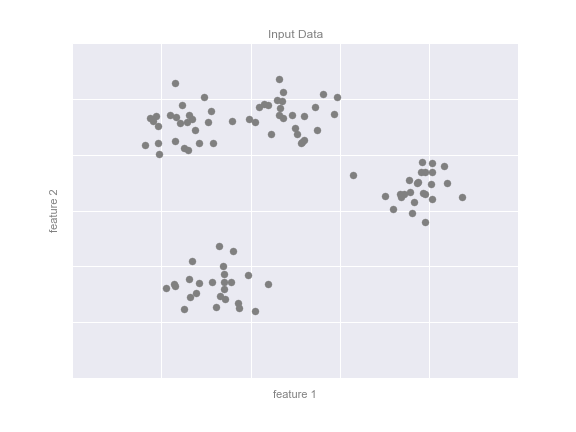
\includegraphics[width=\linewidth]{figs/05.01-clustering-1.png}
 	   \column{.50\textwidth}
			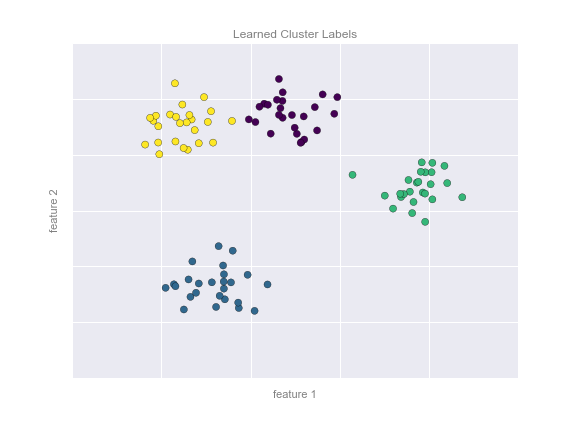
\includegraphics[width=\linewidth]{figs/05.01-clustering-2.png}
    \end{columns}

    \centering \tiny{\href{https://jakevdp.github.io/PythonDataScienceHandbook/05.01-what-is-machine-learning.html}{(Source)}}
\end{frame}

\begin{frame}{Types of Machine Learning systems}{Unsupervised learning: Clustering (II)}
	Example: Cluster word-sentence length in a books corpus

    \begin{columns}
 	   \column{.30\textwidth}
 	   \column{.40\textwidth}
			\begin{figure}
			\centering{
			\resizebox{\textwidth}{!}{\input{figs/cluster.pdf_tex}}}
			\end{figure}
 	   \column{.30\textwidth}
    \end{columns}

	Clusters interpretation
	\begin{itemize}
		\item Long words and sentences: Philosophy?
		\item Short words and sentences: Novel?
	\end{itemize}
\end{frame}

\begin{frame}{Types of Machine Learning systems}{Unsupervised learning: Clustering (III)}
	Example: Human resources department wants to know their employees profiles

	\begin{center}
	\begin{tabular}{ccccccccc}\hline
		 Salary & Married & Car & Child. & Rent/owner & Syndicated & Leaves & Sen. & Sex \\\hline
		 1000   & Yes     & No  & 0      & Rent       & No         & 7      & 15   & M   \\
		 2000   & No      & Yes & 1      & Rent       & Yes        & 3      & 3    & F   \\
		 1500   & Yes     & Yes & 2      & Owner      & Yes        & 5      & 10   & M   \\
		 3000   & Yes     & Yes & 1      & Rent       & No         & 15     & 7    & F   \\
		 1000   & Yes     & Yes & 0      & Owner      & Yes        & 1      & 6    & M   \\
		 %$\cdots$ & $\cdots$ & $\cdots$ & $\cdots$   & $\cdots$  & $\cdots$ & $\cdots$ \\
		 \hline
	 \end{tabular}
	 \end{center}
\end{frame}

\begin{frame}{Types of Machine Learning systems}{Unsupervised learning: Clustering (IV)}

	\begin{center}
	\begin{tabular}{ccccccccc}\hline
				    & \texttt{Group 1} & \texttt{Group 2} & \texttt{Group 3} \\\hline
		 Salary     & 1535    		   & 1428             & 1233       \\
		 Married    & 77\%    		   & 98\% 			  & 0\%        \\
		 Car        & 82\%    		   & 1\% 			  & 5\%        \\
		 Child.     & 0.05    		   & 0.3 			  & 2.3        \\
		 Rent/owner & 99\%    		   & 75\% 			  & 17\%       \\
		 Syndicated & 80\%    		   & 0\% 			  & 67\%       \\
		 Leaves     & 8.3     		   & 2.3 			  & 5.1        \\
		 Seniority  & 8.7     		   & 8 				  & 8.1        \\
		 Sex (M/F)  & 61\%    		   & 25\% 			  & 83\%       \\
		 \hline
	 \end{tabular}
	 \end{center}
	 Analysis:
	 \begin{itemize}
	 	\item Group 1: No children, with rented house. Low syndication. Many sick leaves.
		\item Group 2: No children, with car. High syndication. Low sick leaves. Usually women and rent.
		\item Group 3: With children, married, with car. Usually owners men. Low syndication.
	 \end{itemize}	
\end{frame}

\begin{frame}{Types of Machine Learning systems}{Unsupervised learning: Clustering (V)}
	Example: Cells number count

	\bigskip

	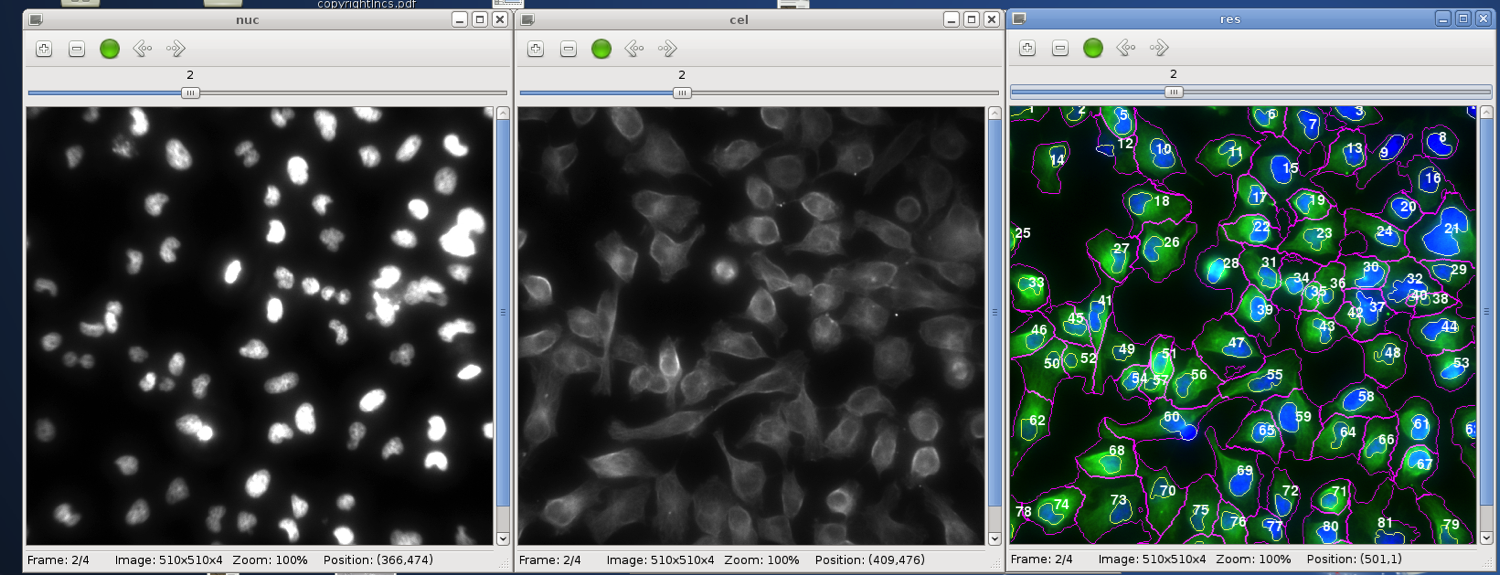
\includegraphics[width=\linewidth]{figs/cellsunsupervised.png}
\end{frame}

\subsection{Association rules}
\begin{frame}{Types of Machine Learning systems}{Unsupervised learning: Association rules (I)}
	Association rules seek relations among attributes

	\begin{center}
	\begin{tabular}{ccccc}\hline
		 $f_1$     & $f_2$     & $f_3$     & $\cdots$ & $f_n$     \\\hline
		 $a_{1,1}$ & $a_{2,1}$ & $a_{3,1}$ & $\cdots$ & $a_{n,1}$ \\
		 $a_{1,2}$ & $a_{2,2}$ & $a_{3,2}$ & $\cdots$ & $a_{n,2}$ \\
		 $a_{1,3}$ & $a_{2,3}$ & $a_{3,3}$ & $\cdots$ & $a_{n,3}$ \\
		 $a_{1,4}$ & $a_{2,4}$ & $a_{3,4}$ & $\cdots$ & $a_{n,4}$ \\
		 $a_{1,5}$ & $a_{2,5}$ & $a_{3,5}$ & $\cdots$ & $a_{n,5}$ \\
		 \hline
	 \end{tabular}
	 \end{center}

	 Main association algorithms
	 \begin{itemize}
	 	\item Apriori, Eclat, GP-growth
	 \end{itemize}
	 Algorithm output
	 \begin{itemize}
	 	\item Rules
		\item Confidence: How often the rule is true 
		\item Support: How often the rule applies 
	 \end{itemize}
\end{frame}

\begin{frame}{Types of Machine Learning systems}{Unsupervised learning: Association rules (II)}
	Example: Market basket analysis
	\begin{itemize}
		\item A supermarket wants to gather information about its clients shopping behaviour
	\end{itemize}

	Objective
	\begin{itemize}
		\item Identify complementary items
		\item Enhance product placement
	\end{itemize}

	\vspace{-0.3cm}

	\begin{center}
	\begin{tabular}{cccccccccc}\hline
		 Id & Eggs & Oil & Diapers & Wine & Milk & Butter & Salmon& Lettuce & $\cdots$ \\\hline
		 1  & Yes  & No  & No      & Yes  & No   & Yes    & Yes   & Yes  & $\cdots$ \\
		 2  & No   & Yes & No      & No   & Yes  & No     & No    & Yes  & $\cdots$ \\
		 3  & No   & No  & Yes     & No   & Yes  & No     & No    & No   & $\cdots$ \\
		 4  & No   & Yes & Yes     & No   & Yes  & No     & No    & No   & $\cdots$ \\
		 5  & Yes  & Yes & No      & No   & No   & Yes    & No    & Yes  & $\cdots$ \\
		 6  & Yes  & No  & No      & Yes  & Yes  & Yes    & Yes   & No   & $\cdots$ \\
		 7  & No   & No  & No      & No   & No   & No     & No    & No   & $\cdots$ \\
		 8  & Yes  & Yes & Yes     & Yes  & Yes  & Yes    & Yes   & No   & $\cdots$ \\
		 $\cdots$ & $\cdots$ & $\cdots$ & $\cdots$   & $\cdots$  & $\cdots$ & $\cdots$ & $\cdots$ & $\cdots$ & $\cdots$ \\
		 \hline
	 \end{tabular}
	 \end{center}
\end{frame}

\begin{frame}[fragile]{Types of Machine Learning systems}{Unsupervised learning: Association rules (IV)}
    \begin{columns}
	   \column{.15\textwidth}
	   \column{.70\textwidth}
	   		\begin{exampleblock}{Association rules}
	   		\begin{lstlisting}[firstnumber=1, xleftmargin=10pt] 
if diapers=yes
then milk=yes (100%, 37%)

if eggs=yes
then oil=yes (50%, 25%)

if wine=yes
then lettuce=yes (33%, 12%)
           \end{lstlisting}
	   		\end{exampleblock}

 		where (confidence, support)
	   \column{.15\textwidth}
	\end{columns}
\end{frame}

\begin{frame}{Types of Machine Learning systems}{Unsupervised learning: Dimensionality reduction (I)}
	Dimensionality reduction transforms data into more convenient representations
	\begin{itemize}
		\item Reduce data dimensionality
		\item Visualize multidimensional data
	\end{itemize}

	Main algorithms
	\begin{itemize}
		\item Isomap
		\item Principal Components Analysis (PCA)
		\item T-distributed Stochastic Neighbor Embedding (t-SNE)
	\end{itemize}
\end{frame}

\subsection{Dimensionality reduction}
\begin{frame}[fragile]{Types of Machine Learning systems}{Unsupervised learning: Dimensionality reduction (II)}
	Example: Isomap

    \begin{columns}
 	   \column{.50\textwidth}
			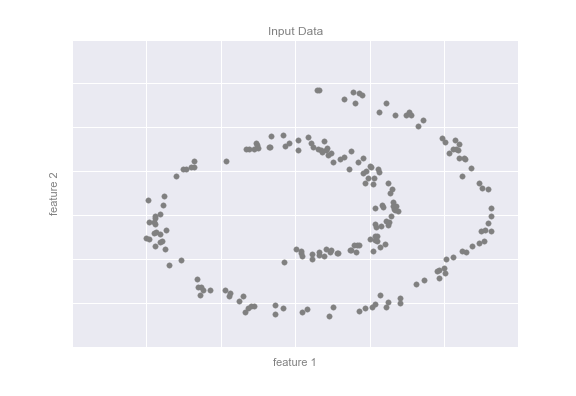
\includegraphics[width=\linewidth]{figs/05.01-dimesionality-1.png}
 	   \column{.50\textwidth}
			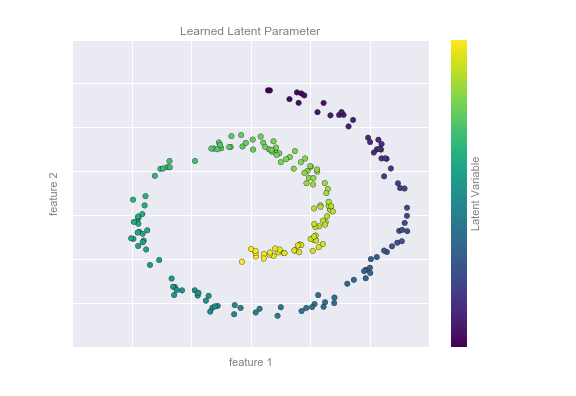
\includegraphics[width=\linewidth]{figs/05.01-dimesionality-2.png}
    \end{columns}
    \centering \tiny{\href{https://jakevdp.github.io/PythonDataScienceHandbook/05.01-what-is-machine-learning.html}{(Source)}}

\end{frame}

\begin{frame}[fragile]{Types of Machine Learning systems}{Unsupervised learning: Dimensionality reduction (III)}
	Example: PCA

    \begin{columns}
 	   \column{.50\textwidth}
			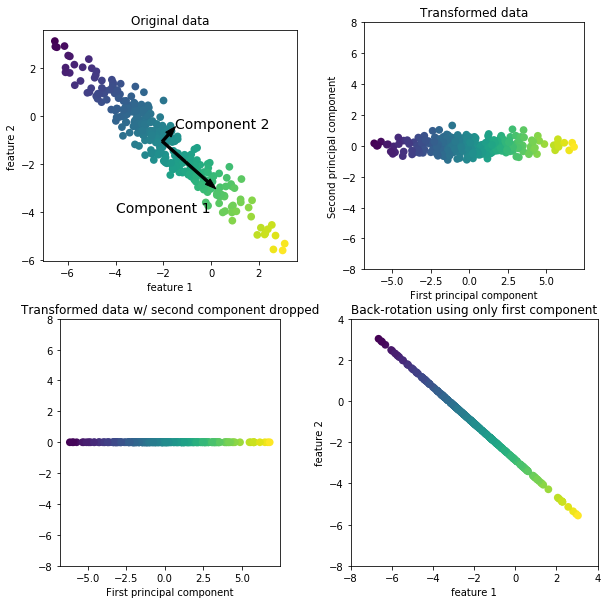
\includegraphics[width=\linewidth]{figs/pca.png}
    		\centering \tiny{\href{https://github.com/amueller/introduction_to_ml_with_python/blob/master/03-unsupervised-learning.ipynb}{(Source)}}
    \end{columns}
\end{frame}

\begin{frame}[fragile]{Types of Machine Learning systems}{Unsupervised learning: Dimensionality reduction (IV)}
	\vspace{-0.5cm}
    \begin{columns}
 	   \column{.70\textwidth}
		Example: Hand-written digits recognition
		\begin{itemize}
			\item Images of hand-written digits
			\item 8x8 images (64 dimensions)
			\item $10$ digits
			\item Classification problem
		\end{itemize}
 	   \column{.30\textwidth}
			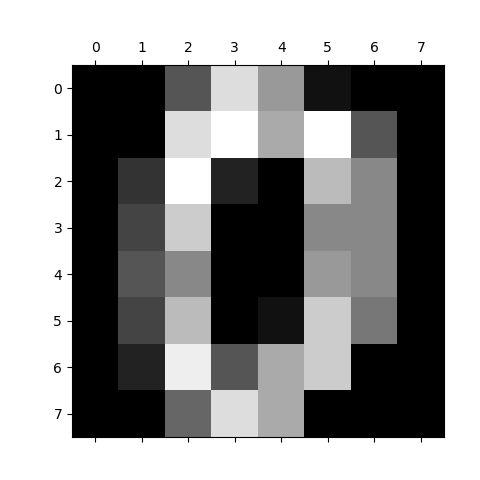
\includegraphics[width=\linewidth]{figs/zero.png}
    \end{columns}

    \begin{columns}
 	   \column{.50\textwidth}
			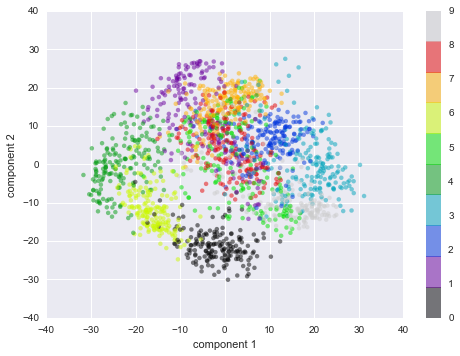
\includegraphics[width=\linewidth]{figs/handdigitspca.png}
 	   \column{.50\textwidth}
			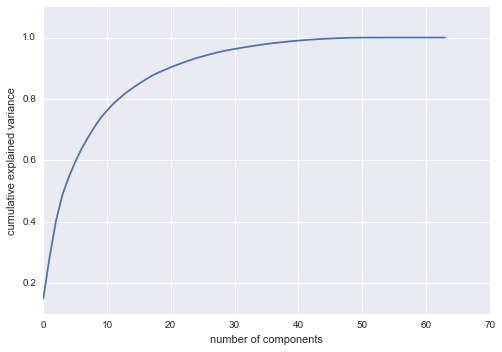
\includegraphics[width=\linewidth]{figs/pcacomponents.png}
    \end{columns}

   	\centering \tiny{\href{https://github.com/amueller/introduction_to_ml_with_python/blob/master/03-unsupervised-learning.ipynb}{(Source)}}
\end{frame}

\section{Main challenges of Machine Learning}

\subsection{Under and overfitting}
\begin{frame}{Main challenges of Machine Learning}{Under and overfitting}
    \begin{columns}
	   \column{.50\textwidth}
		\alert{Underfitting}: Does not learn
            \begin{itemize}
                \item Topology too simple
				\item The model does not fit data
				\item Solution: 
				\begin{itemize}
					\item Increase model complexity
				\end{itemize}
            \end{itemize}

            \begin{center}
			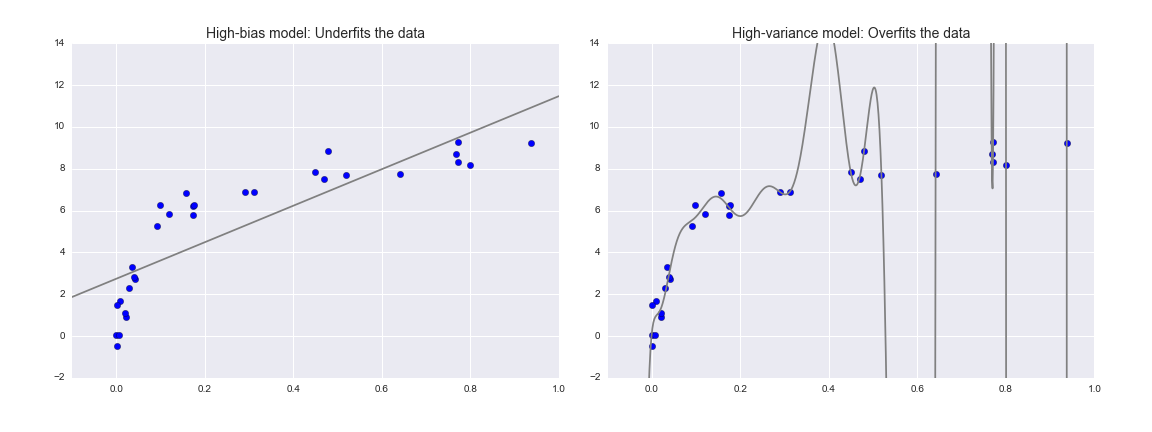
\includegraphics[width=\linewidth]{figs/05.03-bias-variance.png}\\
			\scriptsize \href{https://jakevdp.github.io/PythonDataScienceHandbook/05.03-hyperparameters-and-model-validation.html}{(Source)}
            \end{center}

	   \column{.50\textwidth}
		\alert{Overfitting}: Memorizes samples
            \begin{itemize}
                \item Topology too complex
                \item Very serious concern in ML
				\item The model does not generalize data
                \item Model fails when exposed to new data
				\item Solutions:
				\begin{itemize}
					\item Reduce model complexity
					\item Increase dataset
					\item Apply regularization
				\end{itemize}
            \end{itemize}
   \end{columns}
\end{frame}

\subsection{The curse of dimensionality}
\begin{frame}{Main challenges of Machine Learning}{The curse of dimensionality}
	ML algorithms are statistical by nature
	\begin{itemize}
		\item Count frecuency of observations in regions
	\end{itemize}

	Fewer observations per region as dimensionality increases
	\begin{itemize}
		\item Data become sparser
		\item Need of more data to keep patterns
		\item Increased overfitting risk
	\end{itemize}
	Goal: Reduce dimensionality as much as possible 

	\begin{center}
	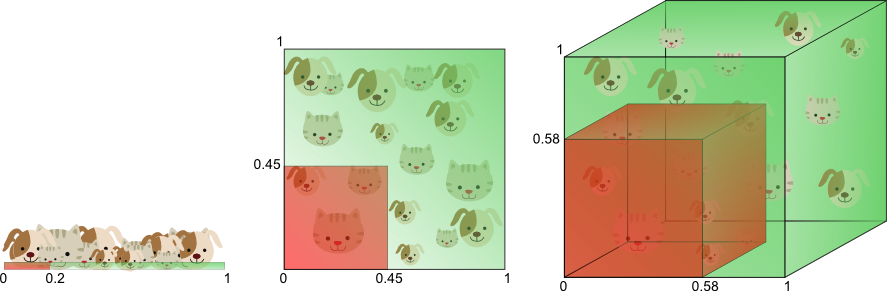
\includegraphics[width=0.8\linewidth]{figs/curseofdimensionality.png}\\
	\tiny{\href{http://www.visiondummy.com/2014/04/curse-dimensionality-affect-classification/}{(Source)}}
   	\end{center} 
\end{frame}

\subsection{Other challenges}
\begin{frame}{Main challenges of Machine Learning}{Other challenges}
	\begin{itemize}
    	\item Insufficient data
			\begin{itemize}
				\item Given enough data, algorithms tend to similar performance
				\item Remember: ML is data-centric
			\end{itemize}
		\item Non representative training data
		\item Poor quality data
		\item Irrelevant features
        \item Unbalanced datasets
    \end{itemize}
	
	\bigskip
	\begin{center}
	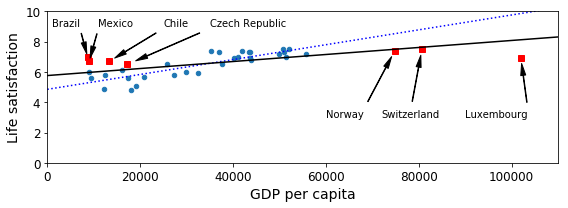
\includegraphics[width=0.6\linewidth]{figs/trainingsample.png}\\
    \tiny{\href{https://github.com/ageron/handson-ml/blob/master/01_the_machine_learning_landscape.ipynb}{(Source)}}
	\end{center}
\end{frame}

\section{Case studies}

\subsection{Bank propensity model}
\begin{frame}{Case studies}{Case study 1: Bank propensity model}
	Client
	\begin{itemize}
		\item Bank
	\end{itemize}
	Business problem
	\begin{itemize}
		\item Identify those clients prone to buy a service
	\end{itemize}
	Data
	\begin{itemize}
		\item Available on several databases
		\item Historical data on service adquisition available
	\end{itemize}
	Propose a solution to:
	\begin{itemize}
		\item Data adquisition
		\item ML task
		\item Predictive or explicative model
		\item Model explotation
		\item Model maintenance
	\end{itemize}
\end{frame}

\subsection{Social media campaign impact}
\begin{frame}{Case studies}{Case study 2: Social media compaign impact}
	Client
	\begin{itemize}
		\item Car manufacturer
	\end{itemize}
	Business problem
	\begin{itemize}
		\item Real-time analysis of a campaign impact in Twitter
		\item Answer if people have a positive reaction to the campaign
	\end{itemize}
	Data
	\begin{itemize}
		\item None
	\end{itemize}
	Propose a solution to:
	\begin{itemize}
		\item Data adquisition
		\item ML task
		\item Predictive or explicative model
		\item Model explotation
		\item Model maintenance
	\end{itemize}
\end{frame}

\subsection{Hubble FGS-3 servo failure prediction}
\begin{frame}{Case studies}{Case study 3: Hubble FGS-3 servo failure prediction}
    \begin{columns}
 	   \column{.50\textwidth}
	   \small{
		Client
		\begin{itemize}
			\item NASA
		\end{itemize}
		Business problem
		\begin{itemize}
			\item Predict Hubble FGS-3 servo failure
		\end{itemize}
		Data
		\begin{itemize}
			\item Compensated error telemetry 
			\item Servo will fail if compensated error exceeds a threshold
		\end{itemize}
		Propose a solution to:
		\begin{itemize}
			\item ML task
			\item Predictive or explicative model
			\item Model explotation
			\item Model maintenance
		\end{itemize}
		}
 	   \column{.50\textwidth}
			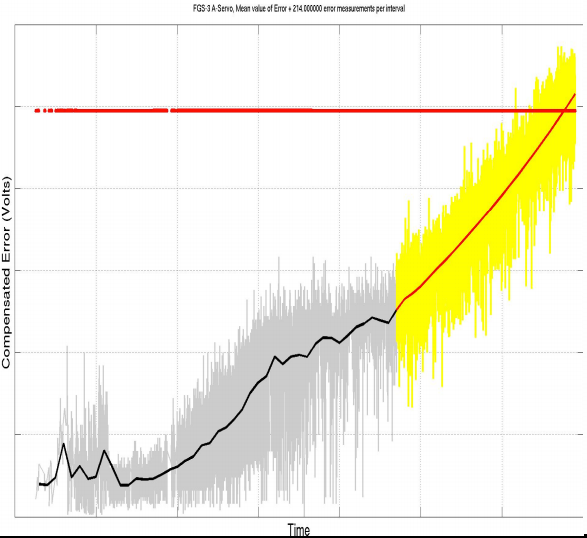
\includegraphics[width=\linewidth]{figs/hubble.png}

			\tiny \centering \href{https://ti.arc.nasa.gov/m/groups/machinelearningworkshop2017/MLW2017_slides/presentationsPDF/Hamed-Valizadegan.pdf}{(Source of this study case)}
    \end{columns}
\end{frame}

\subsection{Fall detection with accelerometer}
\begin{frame}{Case studies}{Case study 4: Fall detection with triaxial accelerometer}
    \begin{columns}
 	   \column{.50\textwidth}
	   \small{
		Client
		\begin{itemize}
			\item Technological start-up
		\end{itemize}
		Business problem
		\begin{itemize}
			\item Detect falls with a smartwatch
			\item Improve elderly people attention
		\end{itemize}
		Data
		\begin{itemize}
			\item None
		\end{itemize}
		Propose a solution to:
		\begin{itemize}
			\item Data adquisition
			\item ML task
			\item Data preprocessing
			\item Model explotation
			\item Model maintenance
		\end{itemize}
		}
 	   \column{.50\textwidth}
			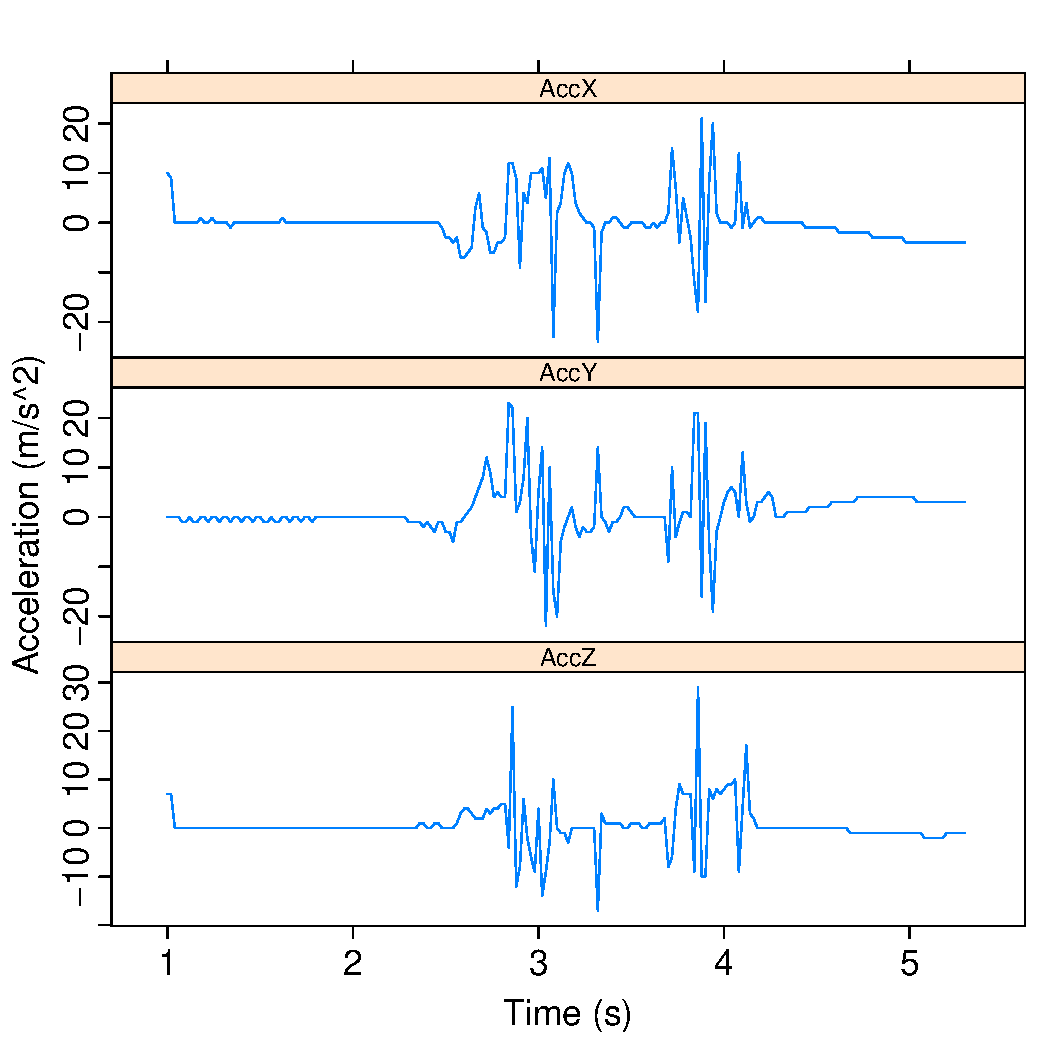
\includegraphics[width=\linewidth]{figs/HFall.pdf}

			\centering \href{https://www.slideshare.net/DavidFBarrero/triaxial-accelerometer-located-on-the-wrist-for-elderly-peoples-fall-detection}{(More info)}
    \end{columns}
\end{frame}

\subsection{Fall detection with sound}
\begin{frame}{Case studies}{Case study 5: Fall detection with sound}
    \begin{columns}
 	   \column{.50\textwidth}
	   \small{
		Client
		\begin{itemize}
			\item Technological start-up
		\end{itemize}
		Business problem
		\begin{itemize}
			\item Detect falls with sound
			\item Improve elderly people attention
		\end{itemize}
		Data
		\begin{itemize}
			\item None
		\end{itemize}
		Propose a solution to:
		\begin{itemize}
			\item Data adquisition
			\item ML task
			\item Data preprocessing
			\item Model explotation
			\item Model maintenance
		\end{itemize}
		}
 	   \column{.50\textwidth}
			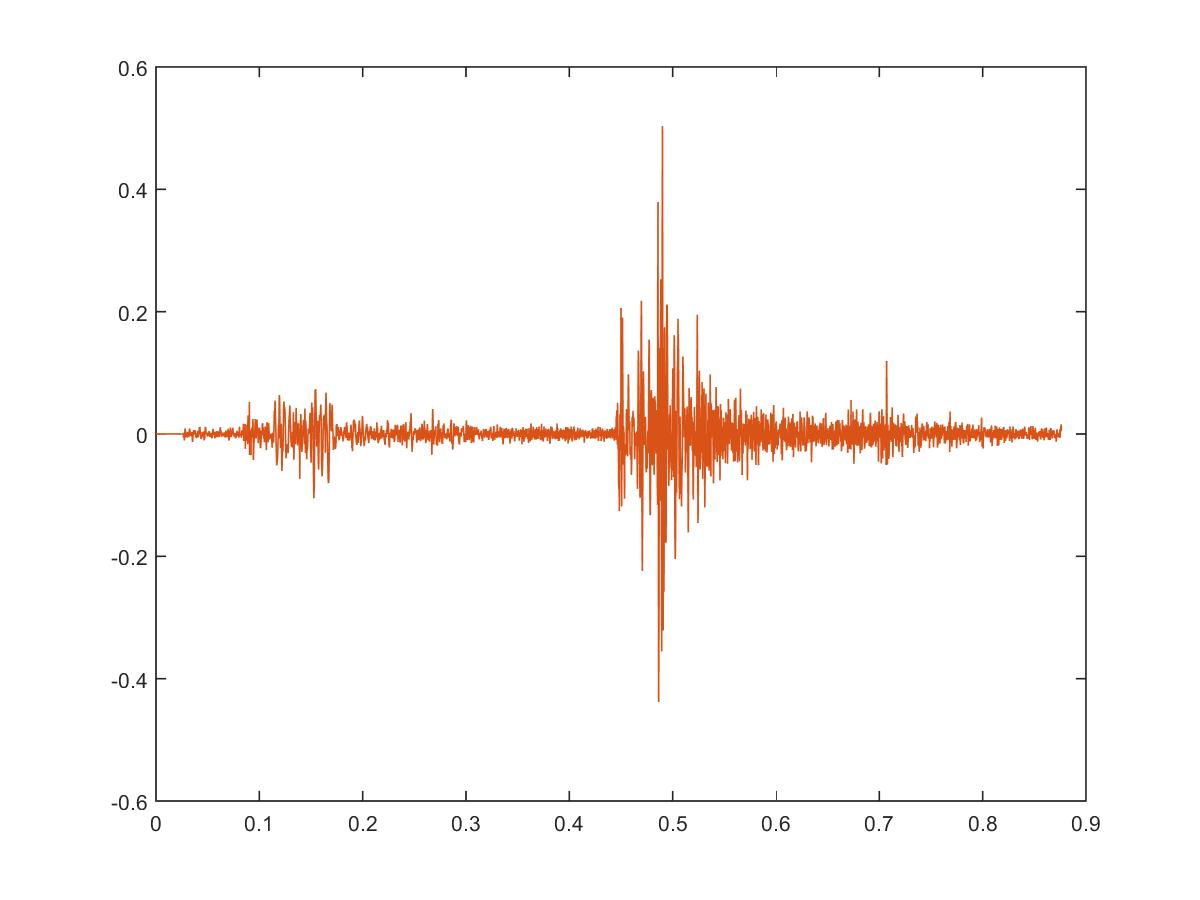
\includegraphics[width=\linewidth]{figs/sound.jpg}

			\footnotesize{
			\begin{tabular}{ll}
			\hline 
			Energy Mean & Energy Std \\
			Number of Zeros Mean & Number of Zeros Std \\
			Spectral Flux Mean & Spectral Flux Std \\
			Roll off Factor Mean & Roll off Factor Std \\
			Spectral centroid Mean & Spectral Centroid Std \\
			\hline
			\end{tabular} 
			}
			
			\centering \href{https://link.springer.com/chapter/10.1007/978-3-319-60042-0_18}{(More info)}
    \end{columns}
\end{frame}

\subsection{NASA JPL BioSleeve}
\begin{frame}{Case studies}{Case study 6: NASA JPL BioSleeve}
	\vspace{-0.5cm}
    \begin{columns}
	   \column{.50\textwidth}
	   \small{
		Client
		\begin{itemize}
			\item NASA JPL Advanced Robotics Group
		\end{itemize}
		Business problem
		\begin{itemize}
			\item Recognize hand gestures \href{https://spectrum.ieee.org/automaton/robotics/robotics-hardware/jpl-biosleeve-enables-precise-robot-control-through-hand-and-arm-gestures}{(more info)}
		\end{itemize}
		Data
		\begin{itemize}
			\item None
		\end{itemize}
		Propose a solution to:
		\begin{itemize}
            \item Data adquisition
			\item ML task
		\end{itemize}
		}

 	   \column{.50\textwidth}
			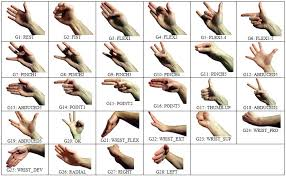
\includegraphics[width=\linewidth]{figs/biosleeve.jpeg}\\
			\tiny \centering \href{https://dces.essex.ac.uk/staff/hhu/Papers/CTS2013-San\%20Diego.pdf}{(Source)}

			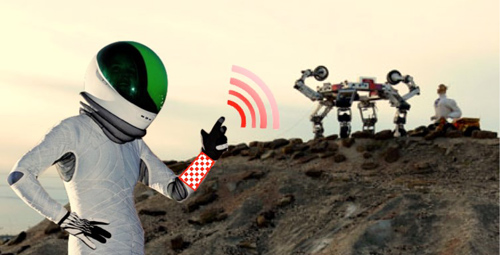
\includegraphics[width=0.5\linewidth]{figs/biosleeve2.jpg}\\
			\tiny \centering \href{https://www-robotics.jpl.nasa.gov/tasks/showBrowseImage.cfm?TaskID=277&tdaID=700081}{(Source)}
    \end{columns}

    \normalsize \href{https://dl.acm.org/citation.cfm?id=2447571}{Wolf, Michael T., et al. \textit{Decoding static and dynamic arm and hand gestures from the JPL BioSleeve}. IEEE Aerospace Conference. IEEE, 2013.}\\

	\vspace{0.3cm}

    \centering \href{https://www.semanticscholar.org/paper/JPL-BioSleeve-for-gesture-based-control\%3A-Technology-Assad-Wolf/18152a964e128e247a706dc8729036369b536b48/figure/2}{(Solution)} \href{https://www.youtube.com/watch?v=BGfDyqAE86U}{(Results)}
\end{frame}

\subsection{UAV terrain classification}
\begin{frame}{Case studies}{Case study 7: UAV terrain classification}
		Client
		\begin{itemize}
			\item NASA JPL Advanced Robotics Group
		\end{itemize}
		Business problem
		\begin{itemize}
			\item Recognize terrain type for automatic UAV landing
			\item \href{https://www.youtube.com/watch?v=ovtpwxiIr_8}{(Video)}
		\end{itemize}
		Data
		\begin{itemize}
			\item UAV down-looking camera
			\item No dataset available
		\end{itemize}
		Propose a solution to:
		\begin{itemize}
			\item Data adquisition
			\item ML task
            \item Feature extraction
		\end{itemize}
\end{frame}

\end{document}
